\chapter{Introduction and Motivation}
\label{introchap}
\section{Asteroid Surfaces} 
Studying asteroids is important to understanding the origin of our own planet. They are remnants of the protoplanetary disk, and provide insights as to the composition of the original materials that eventually formed rocky planets as well as gaseous ones. In this work, I will be focusing on the smallest members of the asteroid population and the unique dynamics at play in their evolution. We will discuss their composition, dynamics, and environmental concerns for imaging in a navigation context. Their shapes are unique and studying them provides much deeper context to the forces that made up our own planet. Refining the forces that influence these asteroids today can also improve our orbit estimates and give better predictions of what asteroids are potentially hazardous. 

Small asteroids are often made up of many separate particles and boulders which is why they are referred to as "rubble piles" \cite{Scheeres2018}. Often originating from a previous impact event of a parent body, the many pieces come together over time and bond by weak gravity and electrostatic cohesion \cite{Walsh2018}. These bodies are resilient and active, frequently resurfacing, losing particles, and experiencing further bombardment. By our recent visits to asteroid targets in the sub-1 km size regime, we have seen high-resolution examples of these bodies and been able to characterize the boulders and regolith on their surfaces. These missions produced shape models that enabled both science and navigation. The OSIRIS-REx mission successfully orbited around the ~492 m diameter asteroid Bennu for two years, measuring the gravitational properties and taking images to constrain the shape \cite{Scheeres2019}. We observed the extremely dark and unexpectedly rocky surface of Bennu and even witnessed particle escape \cite{Hergenrother2019}. The sample taken from Bennu has already returned to Earth to undergo testing and characterization which will tell us more about the materials we should expect to find on B-type asteroids like Bennu in the future \cite{Lauretta2023}. Another recent mission that demonstrated the capabilities of asteroid rendezvous and high-resolution shape modeling was Hayabusa2, launched by JAXA to arrive at Itokawa in 2018 \cite{Watanabe2019}. This mission characterized the irregularly shaped body Itokawa and also furthered asteroid science in unexpected ways. One way includes the expansion of YORP theory and also furthering evidence of the presence of contact binaries in the near-earth asteroid population. i
%any more interesting properties of the surface that I can blurt out?

\subsection{Shape Modeling}
The accurate capture of the surface and bulk shape is an important data product for science and navigation. It enables the precise mapping of the gravity field, and better target characterization for relative navigation solutions (expand this) (cite it). One method for creating a shape model is by the combination of optical images which capture various poses and features of the target body. 


When spacecraft are deployed to study small bodies in our solar system, they lose the consistent ability to access classical systems for communication such as the Deep Space Network which relays messages from the ground-based operators. However, as the sensitivity of the actions executed by these spacecraft increases, such as during the Touch-And-Go maneuver that OSIRIS-REx achieved when sampling the surface of Bennu \cite{Berry2013}, autonomy becomes critical. With radio communications, there is a delay of minutes between sending commands and their execution time which can mean the difference between a landing and a large miss when targeting small bodies for rendezvous or even flybys. This necessary level of autonomy can be achieved by allowing for the onboard processing capabilities that enable navigation and mission-related decision making. Optical information is the primary focus of this study for its advanced development in navigating spacecraft \cite{Owen2011}, despite it's challenges in the space environment \cite{DellaGiustina2018}, where careful planning is required to handle the varying lighting conditions. This work focuses on the construction of the shape model data product during the approach trajectory phase when the body has many pixels of resolution and the silhouette is discernible. This moves away from feature-focused shape modeling approaches such as SPC \cite{Gaskell2008}, stereophotogrammetry (shape from motion)\cite{Hartley2000}, and many other algorithms which identify shadows, craters, rocks and boulders, and even ridges in order to inform the shape. These alternate methods use specific feature detector algorithms to identify surface variations mathematically \cite{Lowe2004}. It is simpler to take advantage of the contrast of a high-albedo body versus a background of space in order to extract a silhouette which can be identified as the limb and terminator of the observable surface. The capabilities accessed via this data type have been shown in previous limb-focused localization approaches by Christian \cite{Christian2017}. 
%image goes here to break up the intro?

Silhouette-based methods of shape modeling are used extensively for the reconstruction of singular objects in the computer vision community\cite{Franco2009}\cite{Matusik2000}\cite{Boyer2003}. As the small-body community encounters a similar problem, there is a push to investigate limb information as a solution to onboard processing limitations \cite{Panicucci2020}\cite{Liounis}. A limb refers to the contour of the edge of the body on the lit side and is differentiated from the background of space. A shape such as an asteroid or a binary system is a good candidate and many variations of these natural shapes have been investigated by previous studies. Alongside simulated tool development, these practices have been applied in-house for mission data solutions. The OSIRIS-REx mission developed and applied a limb-based tool (LIMBER) to resolve a pre-SPC model with accuracy of 3-4m when image frequency was $~10^{\circ}$ and the spacecraft was located in a hovering position within 200km from the target \cite{Palmer2019}. Their approach followed very similar procedure as the work presented here, but was not able to apply information from the terminator. Other teams have focused on a similarly simulated method based on finding the silhouette and carving the 3D shape from a preset voxel cube \cite{Bandyonadhyay2019}. The aim of each of these efforts is to show that the silhouette information is both robust and computationally efficient as a candidate for onboard processing. Previous work has highlighted the requirements of the image processing stage when sourcing limb information from optical data \cite{Li2013}. The shape model built using approach observations in the optical range can reach a precision level high enough for navigation purposes with few assumptions at the current stage of development. The future goal is to evolve a dynamic shape model stored onboard, which can be used to inform future navigation decisions; this would improve the overall mapping performance, heightening the autonomy of the mission \cite{Pesce2018}.  


%cut this, put it in chapter 2
In this work, the models presented are generated from simulated data sources and compared to the most resolute shape models available for the bodies in question. The method is tested on both a convex and irregular body in order to show how our overlaid silhouette trimming procedure responds to self-shadowing, the presence of concavity, as well as phase angle projections of the terminator introduced by the orientation of the sun and camera. This algorithm will be developed as necessary to enable onboard shape model generation, but this paper serves to present and defend the method which uses a process of refinement based on extending the shape along the silhouette cutout in space, and narrowing down the three-dimensional hull through multiple viewing angles. As the small body community looks to grant more SIMPLEx-level missions to asteroids,  it is necessary to develop the autonomous onboard navigation capabilities that make those missions possible. 


\subsection{Dynamics and the YORP Effect}
Small bodies in our solar system and particularly in the near-earth environment are of interest to scientists for their resources, their connection to the proto-planetary origins of our Earth, and the possible threat of impact with our planet. Many factors make this population difficult to characterize, such as their limited size, low albedo surfaces, and the difficulty of predicting precise orbits due to low frequency of observation and unmodeled forces. Collective survey efforts have yielded a possible $30\%$ of the >100m population found while the rest remain undiscovered. Observation efforts are increased each year in order to increase the database of known bodies and also our confidence in the dynamics of dangerous suspects that could intersect with our own planet's orbit \cite{Jones2016}\cite{Mainzer2011}. These efforts reveal new targets for space missions that aim to flyby or rendezvous with small bodies to learn more about their surfaces and possibly conduct sample return for deeper Earth-based compositional analysis. In any case, the entire size range of small bodies is of high interest to the scientific and planetary defense communities. This work focuses on the smallest members of the asteroid population, bodies under 1km in diameter, and the particular thermal interactions changing their orbit in ways that have only recently been observed. We have just discussed the motivation towards shape modeling for navigation purposes, and now we will apply what is known of these shapes towards further understanding of the dynamics of small bodies as a whole. =

The Yarkovsky-O'Keefe-Radzievskii-Paddack (YORP) effect is a force that becomes dominant for asteroids with a diameter below one kilometer. This is a radiation recoil force that acts to change the spin rate and pole orientation via asymmetries in the shape of a body. The surface imparts additional torque during the process of absorbing and re-radiating thermal energy that applies secular forces over the course of it's rotational day and year. The surface asymmetries of the body contribute to the change in the spin rate, either spinning the body up or down depending on the bias of the features. Spin-pole obliquity change occurs due to global deviations in symmetry, imparting a tilt on the spin axis which could eventually lead to tumbling. Note that the YORP effect is acting purely on the local attitude of the body via interactions with the surface and it's irregularities, while the Yarkovsky effect acts on all bodies to cause a change in the semi-major axis of the orbit due to the thermal inertia that retains solar heating and emits it at a different phase angle\cite{Vokrouhlicky2000}. We have thus far observed 12 bodies in our solar system that exhibit dynamical changes due to YORP \cite{Durech2023}. This is due to the increase in efforts to observe and model the YORP effect. It is shown that YORP is extremely sensitive to small-scale topography such as boulders and craters on the surface, or even a smaller approximation of surface roughness through regolith modeling \cite{Statler2009}\cite{Rozitis2011}\cite{Rozitis2013}. It is of significant interest to characterize YORP accounting for common features of small bodies in the YORP-dominant size regime, such as boulders, craters, and regolith \cite{Zhou2023}\cite{Walsh2019}. We choose to investigate the populations and properties of boulders. 


Boulders have geological significance because they hold information about local surface processes and natural movement of materials \cite{Murdoch2015}. For the case of small bodies, we assume boulder motion is due to local landslides, regolith redistribution from tidal forces or planetary encounters, and surface sublimation causing fracturing \cite{Delbo2022} \cite{Barnouin2022}. The parameters of size, shape, texture, and comparative composition are all indicators of the time history of geological evolution for a small body. Boulders have been found on all rubble-pile asteroids and they contribute unique properties thermally, geologically, and dynamically \cite{Kuppers2012}. As fractured protrusions, they absorb and radiate heat tangent to the surface \cite{Golubov2022}. Their continuous motion and degeneration contributes majorly to the changing shape of small bodies \cite{Molaro2020} \cite{Scheeres2015}\cite{Scheeres2018}\cite{Zhang2022}. Lastly, they are a vehicle of energy dissipation via infilling, escape, and aggregation \cite{Holsapple2010}.
Due to the small sample size of observed asteroid surfaces, there is no deterministic way to analyze the boulder distribution on all possible asteroid shapes. The surfaces that are available for analysis come from recent mapping and sample acquisition missions such as OSIRIS-REx which successfully mapped Bennu to a mean accuracy of 30 cm \cite{Bennett2021}. Despite this, the possible shapes of small bodies in our solar system are highly variable and extremely difficult to constrain from ground-based observations. The approach taken in this work is to develop statistical approximations for the size and frequency of boulders on an asteroid surface from the currently available image datasets \cite{DellaGiustina2019}\cite{Fujiwara2006}\cite{Watanabe2019}.

In this work, we will largely focus on calculating the normal YORP torque, produced from the absorption and re-radiation of thermal energy from a facet-approximated surface and an array of boulders artificially included in the shape. Other ways that the YORP effect is observed are in crater YORP and tangential YORP. Tangential YORP is also the result of protrusive features as they allow for the possibility of total thermal acclimation that will result in a pro-spin radiative force. This is because the boulder diameter is less than the thermal skin depth for a body of ideal specific heat, thermal conductivity, and spin rate \cite{Golubov2017}.  





This approximation serves to constrain the possible variability in YORP due to boulders for bodies in these size regimes. Rather than using a purely stochastic approach, the uncertainty is informed by Monte Carlo simulation of a known shape decorated with boulder populations following the distributions modeled after real surfaces. We approach the question of YORP variability from a new direction, using observational data to calculate possible bounds on YORP torque due to the additional presence of boulders.We will characterize the magnitude of YORP spin torque due to a singular boulder in different conditions.
\subsection{Thesis Statement}
The thesis of this work can be summarized with the following statement:

\centering
\textbf{\it{The surface features and shapes of small asteroids influence their own dynamics through thermal interactions of the YORP effect. Simulating natural variations in the surface provides natural results for YORP-induced spin and obliquity evolution. This is necessary for constraining and estimating their orbits for the purpose of enabling safer rendezvous missions and improving future impact predictions}}
\subsection{Thesis Overview}
\subsubsection{Contributions}
This dissertation
\begin{enumerate}
    \item Applies mapping techniques to convex and irregular shaped bodies to improve onboard optical navigation data
    \item Demonstrates methods of image processing for asteroid proximity data
    \item Expands YORP modeling to include mid-size surface features
    \item Quantifies the large effect that realistic boulders may have on YORP dynamics, in the spin and obliquity evolution equations
    \item Compares estimates of low resolution shapes with additional simulated boulders to ground-based measurements of YORP acceleration
    \item Derives a YORP thermal inertia model which considers spin velocity over time
    \item Shows that features over 1/500*$R_{ast}$ in diameter are the influential contributors to YORP evolution at a rate of XXXX times 
    \item Had a good time overall
\end{enumerate}


























%This sample document illustrates how to use the
%{\tt thesis} class, originally written by John P. Weiss.
%Some requirements of the Graduate School are written
%into that file; page size, line spacing, appropriate
%placement of captions for tables and figures, etc.
%Revisions by Hongcheng Ni make it possible to use the
%(optional)
%\verb2\usepackage{hyperref}2 command to enable
%internal hyperlinks in the final PDF document.
%Other tasks of conforming to the requirements are
%left to other existing \LaTeX{} packages.
%For example, a common problem is to insert graphics ---
%figures and tables --- into the body of the thesis.  For
%this one should use the {\tt graphicx} package, which is
%part of the standard \TeX{} distribution.  Likewise, the
%Grad School specs say that a large table may be displayed
%in landscape mode at reduced size, but its caption must
%also be in rotated position, in the same font and size as
%the normal text in the body of the thesis.  To accomplish
%this, the user must invoke the {\tt rotating} package,
%available online.


%Figure \ref{xfigDiagram} shows an image from a PDF file
%imported into this document
%using the \verb2graphicx2 package.
%%The command \verb2\usepackage{graphicx}2, which appears
%near the very top of the main \LaTeX{} file, reads in
%this package which defines the
%\verb2\includegraphics{}2 macro.


%\begin{figure}[htbp]
%	\caption[Cylinder and measurements]{
%	This diagram of a cylinder and various
%	measurements and quantities was actually
%	made using {\bf xfig}, a freeware
%	drawing program for Unix systems.
%	Diagrams can be exported directly to PDF
%	files, the preferred format for
%%	vector graphics.  Vector graphics can
%	be magnified indefinitely without degradation,
%	whereas bitmap images (JPG and PNG)
%	must be pretty high-resolution if you don't
%	want them looking all pixellated when
%	magnified.
%	}
%    \begin{center}
%	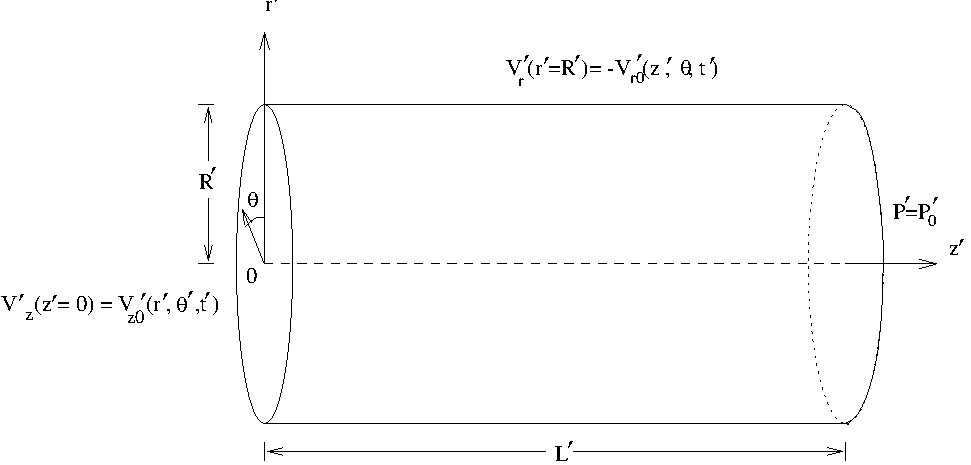
\includegraphics[width=100mm]{figs/cyl.pdf}
%    \end{center}
%\label{xfigDiagram}
%\end{figure}


% \begin{figure}[htbp]
%     \caption[Bitmap images]{
% 	The JPEG bitmap format is great for photos but
% 	crummy for diagrams (including drawings, graphs,
% 	charts) because it can't gracefully handle sharp edges.
% 	Note the same bitmap image below from a PNG file and
% 	from a JPG file; the latter shows characteristic
% 	``ringing'' at sharp edges -- including text!
% 	Seriously, magnify and look closely at the JPG's
% 	awful lines and edges.
% 	Vector-format PDF is the best for diagrams, but
% 	if you must use a bitmap image, let it be PNG.
% 	~ (Left: file {\it drawing.png}.
% 	Right: file {\it drawing.jpg}.)
% 	}
%     \begin{center}
% 	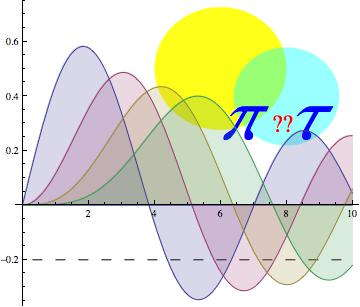
\includegraphics[width=70mm]{figs/drawing.png}
% 	${}^{}$ ~
% 	${}^{}$ ~
% 	${}^{}$
% 	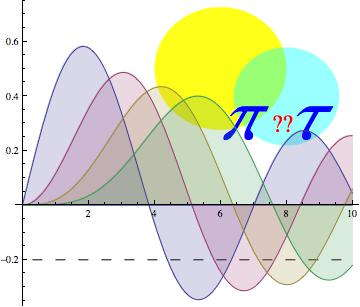
\includegraphics[width=70mm]{figs/drawing.jpg}
%     \end{center}
% \label{bitmapImages}
% \end{figure}



% \section{Lists in {\tt thesis} class}

% In {\tt thesis} class (for Colorado University),
% lists are defined so that nested lists will be
% numbered or marked appropriately.
% First, an itemized (non-enumerated) list
% prefaces each item with a bullet.
% Nested itemized list use asterisks,
% then dashes, then dots.
% These lists are typed between
% the \verb2\begin{itemize}2
% and \verb2\end{itemize}2
% commands.

% \begin{itemize}
%   \item{} This is ``itemized'' item A.
%   \item{} This is ``itemized'' item B.
%   \item{} This is ``itemized'' item C.
%   \begin{itemize}
%     \item{} This is ``itemized'' subitem A.
%     \begin{itemize}
%       \item{} This is ``itemized'' subsubitem A.
%       \begin{itemize}
%         \item{} This is ``itemized'' subsubsubitem A.
%       \end{itemize}
%       \item{} This is ``itemized'' subsubitem B.
%     \end{itemize}
%     \item{} This is ``itemized'' subitem B.
%   \end{itemize}
%   \item{} This is ``itemized'' item D.
% \end{itemize}

% Enumerated lists use the commands
% \verb2\begin{enumerate}2 and
% \verb2\end{enumerate}2,
% and nested enumerations appear like this.

% \begin{enumerate}
%   \item{} This is ``enumerated'' item A.
%   \item{} This is ``enumerated'' item B.
%   \item{} This is ``enumerated'' item C.
%   \begin{enumerate}
%     \item{} This is ``enumerated'' subitem A.
%     \begin{enumerate}
%       \item{} This is ``enumerated'' subsubitem A.
%       \begin{enumerate}
%         \item{} This is ``enumerated'' subsubsubitem A.
%       \end{enumerate}
%       \item{} This is ``enumerated'' subsubitem B.
%     \end{enumerate}
%     \item{} This is ``enumerated'' subitem B.
%   \end{enumerate}
%   \item{} This is ``enumerated'' item D.
% \end{enumerate}


% The work presented
% here\footnote{Footnotes are handled neatly by \LaTeX.}
% is an extension of Lao\cite{lao:thesis}
% and Lao et~al.\cite{lao:paper},
% fictional references that are in the bibliographic
% source file \verb9refs.bib9.

% \begin{table}[htb]
%     \caption[Example of a table with its own footnotes]{
% 	Here is an example of a table with its own footnotes.
% 	Don't use the $\backslash${\tt footnote} macro if you
% 	don't want the footnotes at the bottom of the page.
% 	Also, note that in a thesis the caption goes
% 	\emph{above} a table, unlike figures.
% 	}
%     \begin{center}
%     \begin{tabular}{||l|c|c|c|c||} \hline
% 	& $S$ & $P$ &   $Q^{\ast}$  & $D^{\dagger}$ \\	% footnote symbols!
% 	wave form & (kVA) & (kW) & (kVAr) & (kVAd) \\  \hline \hline
% 	Fig.  \ref{xfigDiagram}a  & 25.48 & 25.00 & -2.82 & 4.03 \\ \hline
% 	Fig.  \ref{xfigDiagram}b  & 25.11 & 18.02 & -9.75 & 14.52 \\ \hline
% 	Table \ref{pdftable}  & 24.98 & 22.26 & 9.19 & 6.64 \\ \hline
% 	Table \ref{powertable}  & 23.48 & 15.00 & 6.59 & 16.82 \\ \hline
% 	Fig.  \ref{pyramid}  & 24.64 & 22.81 & -0.44 & 9.3 \\ \hline
% 	\end{tabular}
%    \\ \rule{0mm}{5mm}
%    ${}^\ast$kVAr means reactive power.		% footnote symbol
% \\ ${}^\dagger$kVAd means distortion power.	% footnote symbol
% \end{center}
% \label{powertable}
% \end{table}


